\subsubsection{Expo CLI}
\label{expocli}
Die Entwickler von React Native selbst empfehlen allen Anfängern im Gebiet App-Entwicklung die
Verwendung der Expo CLI \cite{expocli}, welche eine vereinfachte Variante einer React Native Anwendung erzeugt.

Als Vorteil zählt auf jeden Fall die Geschwindigkeit, mit der eine neue App auf einem neuen Gerät
getestet werden kann. Dies ist meist innerhalb weniger Minuten möglich.

Ein wichtiger Nachteil ist jedoch, dass man in einem Expo-Projekt eingeschränkten Zugriff auf
Schnittstellen des Betriebssystems hat, es sind im Projekt nicht einmal die Ordner android und ios
vorhanden, um Änderungen vorzunehmen.

\subsubsection{Installation und Erstellung einer Expo App}
Um eine Expo React Native Anwendung erstellen zu können benötigt man als erstes \nameref{nodejs} und
den darin enthaltenen Node Package Manager. In einer Kommandozeile führt man nun folgende Befehle
aus, um die Expo-CLI im globalen Kontext zu installieren und anschließend ein Expo Projekt zu
erstellen. Nach der Auswahl für die Vorlage wir das Projekt erstellt.

\begin{lstlisting}
C:\example> npm install -g expo-cli
added 1549 packages, and audited 1550 packages in 1m

C:\example>expo init expoInitBlank
? Choose a template: - Use arrow-keys. Return to submit.
    ----- Managed workflow -----
>   blank               a minimal app as clean as an empty canvas
    blank (TypeScript)  same as blank but with TypeScript configuration
    tabs (TypeScript)   several example screens and tabs using react-navigation and TypeScript
    ----- Bare workflow -----
    minimal             bare and minimal, just the essentials to get you started
\end{lstlisting}

\subsubsection{Ordnerstruktur}
\begin{figure}[H]
  \begin{center}
    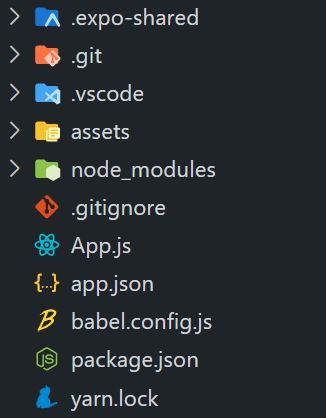
\includegraphics[width=0.5\textwidth]{Theorie/ReactNative/ExpoFolderStructure.JPG}
    \caption{Ordnerstruktur Expo Init Blank}
  \end{center}
\end{figure}

\begin{itemize}
\item Ordner:
\begin{itemize}
\item \textbf{.expo-shared, .git, .vscode}:\\
In den Ordnern .expo-shared, .git und .vscode befinden sich lediglich Konfigurationsdateien für Expo
selbst, die Versionsverwaltungssoftware Git und Visual Studio Code, dem Text-Editor, den wir
durchwegs für die gesamte Diplomarbeit verwendet haben.

\item \textbf{assets}:\\
Der Ordner assets ist für das Abspeichern von statischen Ressourcen, wie Bildern, Icons oder
ähnliches gedacht.

\item \textbf{node\_modules/}:\\
Im Ordner node\_modules werden alle Bibliotheken abgespeichert, die mit Hilfe des Paketmanagers
in das Projekt eingebunden wurden. Expo entschied sich gegen die Verwendung von NPM und verwendet
stattdessen Yarn.
\end{itemize}

\newpage

\item Dateien:

\begin{itemize}
\item \textbf{App.js}\\
Die wichtigste Datei im Projekt ist wohl App.js, sie ist der Einstiegspunkt für die App.

\begin{lstlisting}
import { StyleSheet, Text, View } from 'react-native';

function App() {
  return (
    <View style={styles.container}>
      <Text>Open up App.js to start working on your app!</Text>
    </View>
  );
}

const styles = StyleSheet.create({
  container: {
    flex: 1,
    backgroundColor: '#fff',
    alignItems: 'center',
    justifyContent: 'center',
  },
});

export default App;
\end{lstlisting}

In der ersten Zeile des Programms werden diverse React Native Core Components importiert. Core
Components sind, wörtlich übersetzt, die Kernkomponenten des Frameworks, mit ihnen wird der Großteil
der Benutzeroberfläche aufgebaut. Wie bereits erwähnt, werden die React Native Komponenten beim
Kompilieren in die richtigen Komponenten für das Zielsystem umgewandelt.

\begin{table}[H]
\centering
\begin{tabular}{|l|l|l|l|}
  \hline
  \textbf{Komponente} & \textbf{Android} & \textbf{iOS} & \textbf{HTML} \\ \hline\hline
  View                & ViewGroup        & UIView       & div          \\
  Text                & TextView         & UITextView   & p            \\ \hline
\end{tabular}
\end{table}

\begin{center}
  React Native Core Components und deren Äquivalente im Überblick \cite{reactNativeCoreComponents}
\end{center}

In der nächsten Zeile wird unserer erster React-Component erzeugt, welcher im Grunde nur eine
Funktion ist, die \nameref{jsx}-Code als Rückgabewert liefert.

In Zeile 5 wird zur View ein React Native StyleSheet zugewiesen. Man verwendet nämlich kein
gewöhnliches \nameref{css}, wie in der Webentwicklung, sondern ein relativ ähnlich aufgebautes,
eigenes System zur Gestaltung der App. Ein wichtiger Unterschied ist, dass die Attribut-Namen im
StyleSheet nicht durch Bindestriche getrennt, sondern in der LowerCamelCase-Notation geschrieben
werden \cite{camelCaseNotation}.

Am Ende der Datei wird noch die Komponente als Default exportiert, damit sie von Expo verarbeitet
werden kann \cite{jsModules}.

\item \textbf{app.json, package.json}\\
app.json wird von Expo generiert und mit Metadaten befüllt. In ihr werden Daten abgespeichert,
die nicht in der App selbst eingebaut werden, sondern das Projekt selbst beschreiben, z.B. Name der
App, Versionsnummer, Bildschirmausrichtung und noch viele weiter Optionen.

\begin{figure}[H]
  \begin{center}
    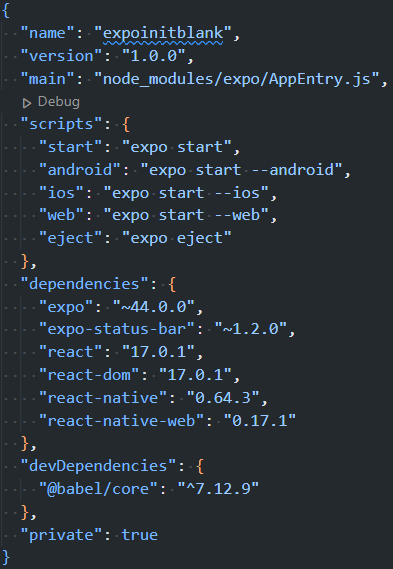
\includegraphics[width=0.5\textwidth]{Theorie/ReactNative/package-json.png}
    \caption{package.json in einem Expo Blank Template}
  \end{center}
\end{figure}

package.json hat einen ähnlichen Zweck, auch darin sind Name, Versionsnummer, aber auch der
Eintrittspunkt in die App abgespeichert. In Scripts werden Kommandozeilenbefehle abgespeichert, die
mit Hilfe des Befehls npm run <script> aufgerufen werden können. Im nächsten Objekt werden die
Namen der Bibliotheken aufgelistet, welche für das Ausführen der App benötigt werden. Bibliotheken,
die nur während der Entwicklung benötigt werden, sind unter devDependencies abzuspeichern (beim
Installieren den Tag -{}-save-dev anhängen).

\item \textbf{package-lock.json, yarn.lock}\\
package-lock.json und yarn.lock haben beide dieselbe Aufgabe, sie sollten jedoch niemals
gleichzeitig im gleichen Projekt existieren. Ersteres gehört nämlich zum Paketmanager NPM, wobei
yarn.lock von Yarn generiert wird. Expo erzeugt ein Blank-Template standardmäßig mit Yarn, man kann
aber auch stattdessen mit dem Tag -{}-npm bei der Projekterstellung NPM einbinden.

\item \textbf{babel.config.js}\\
Babel ist ein sogenannter JavaScript-Transpiler. Er wandelt JavaScript-Features, welche erst in
späteren Versionen des ECMAScript-Standards eingebaut und möglicherweise noch nicht von allen
Systemen unterstützt werden, in JavaScript-Code um, welcher auch von älteren Versionen verstanden
werden kann, um (vgl. ein Compiler wandelt lesbaren Code in Maschinencode um). Außerdem hat er noch
einige andere Funktionen, welche durch Plugins hinzugefügt werden können. In der Konfigurationsdatei
wird nur eine vorgefertigte Liste an Plugins in das Projekt eingebunden, das "babel-preset-expo".

\item \textbf{.gitignore}\\
In die Datei .gitignore fügt man Datei- und Ordnernamen ein, die nicht von der Versionsverwaltung
gesichert werden sollen. Sehr zu empfehlen ist dies beim Ordner node\_modules, da dieser schon
direkt nach der Erstellung 170 Megabytes groß ist und er aus den Dateien package.json und yarn.lock
generiert werden kann.

\end{itemize}
\end{itemize}

\subsubsection{Metro}
\label{metrobundler}
Beim Start der App wird als erstes der Metro Bundler initialisiert. Er besteht aus einem Server,
welcher den geschriebenen Code mittels Babel kompiliert und anschließend an die App schickt. Dadurch
verhindert man, jedes mal die App neu auf das Gerät installieren zu müssen, um eine kleine Änderung
im Text sehen zu können. Beim Einbinden von neuen JavaScript-Bibliotheken muss allerdings der
Bundler neu gestartet werden, um diese verwenden zu können.

Um die App zu starten gibt man folgenden Befehl ein:

\begin{figure}[H]
  \begin{center}
    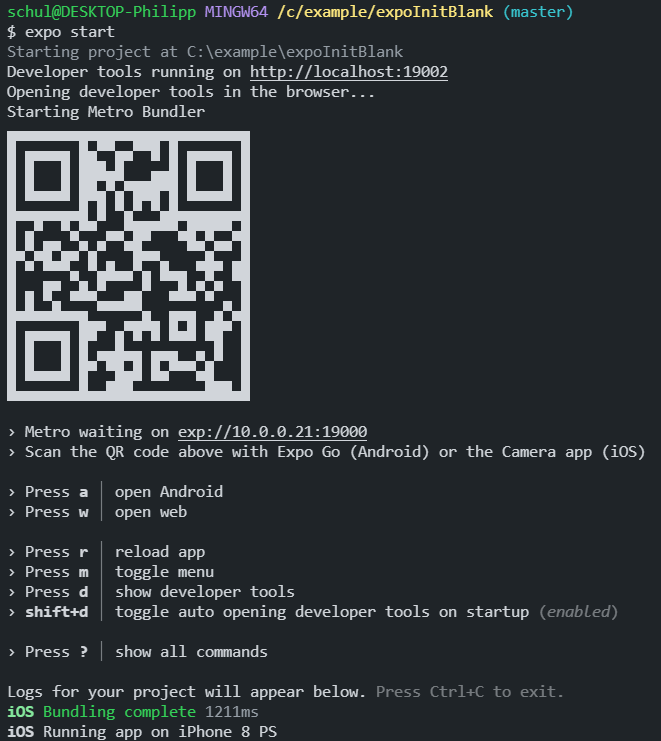
\includegraphics[width=0.6\textwidth]{Theorie/ReactNative/ExpoStart.png}
    \caption{Expo beim Start}
  \end{center}
\end{figure}

\begin{figure}[H]
  \begin{center}
    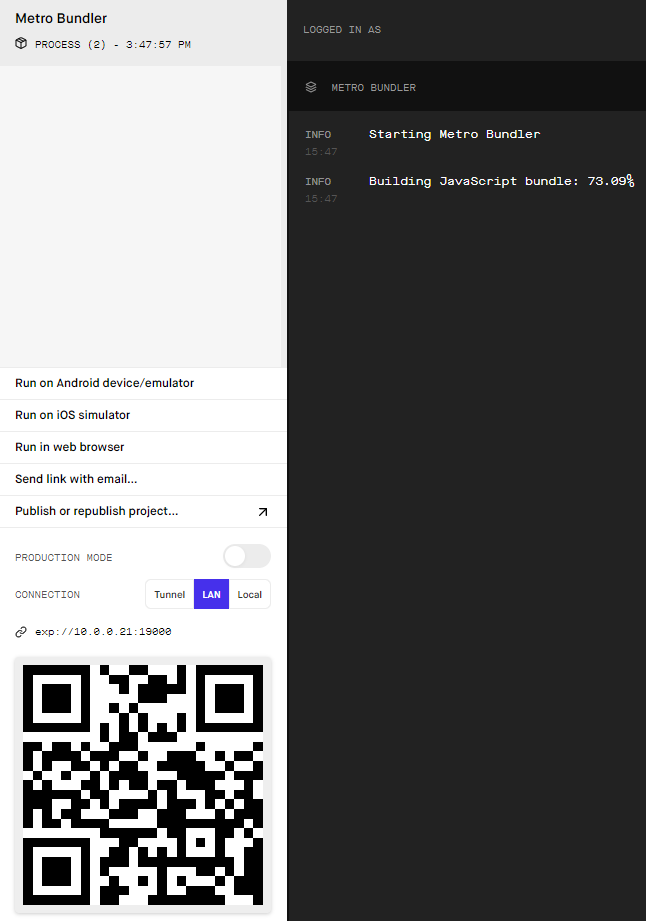
\includegraphics[width=0.6\textwidth]{Theorie/ReactNative/ExpoWebClient.png}
    \caption{Webinterface von Expo}
  \end{center}
\end{figure}

Nach dem Start wird im Webbrowser ein Entwickler-Menü geöffnet, auf dem noch einmal der QR-Code
und noch einige weitere hilfreiche Funktionen zu finden sind.

Um nun die App zu testen, muss man noch die ExpoGo App auf seinem Mobiltelefon installieren und den
gezeigten QR-Code scannen, während man im selben Netzwerk ist. Danach wird eine Bundle-Anfrage an
den lokalen Metro-Server geschickt, er kompiliert unser Projekt und schickt es an den Client.

\begin{figure}[H]
  \begin{center}
    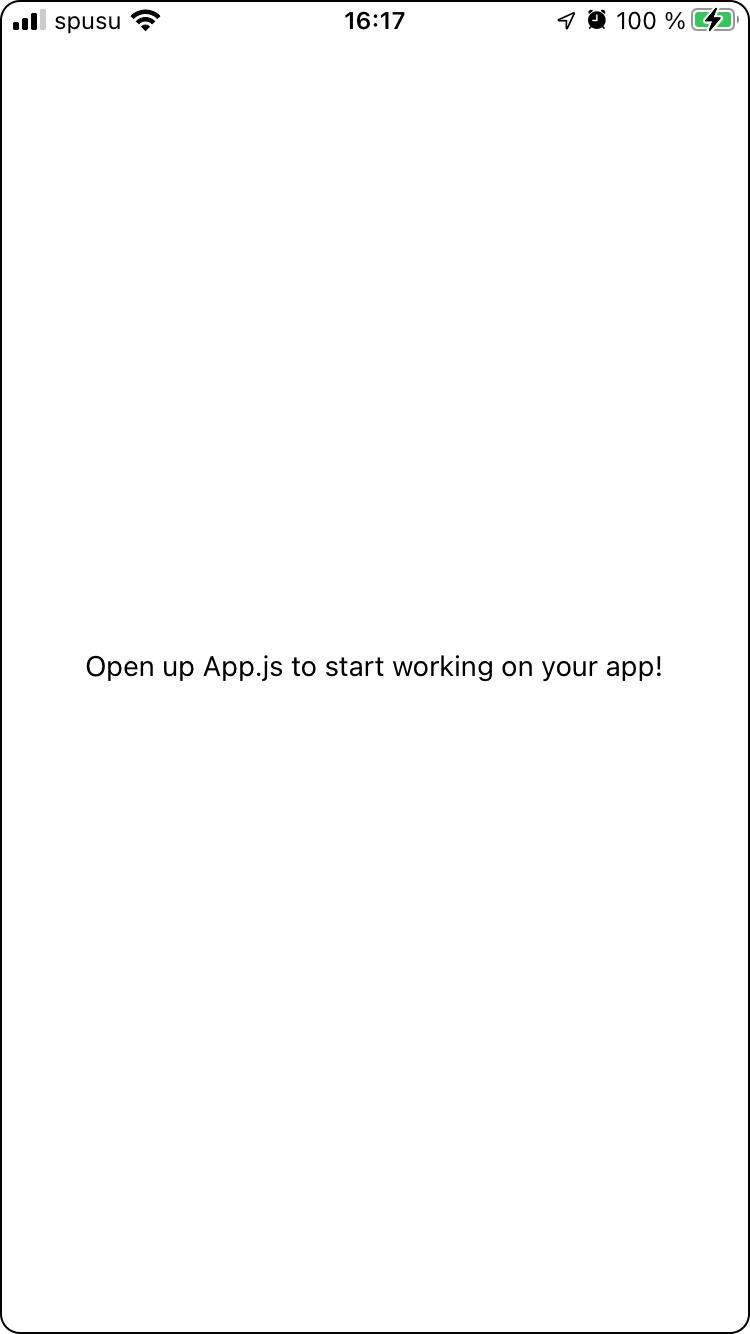
\includegraphics[width=0.5\textwidth]{Theorie/ReactNative/ExpoBlank.jpeg}
    \caption{Die weiße Leinwand von Expo}
  \end{center}
\end{figure}

\subsubsection{Expo Eject}
Wie bereits vorher schon erwähnt, hat es einige Nachteile seine App mit Expo zu machen. Um aber
einen schnellen Prototypen zu bauen ist das Framework perfekt. Um also eine Expo App in eine
vollwertige React Native Anwendung umzuwandeln, benötigt man folgenden Befehl.

\begin{lstlisting}
C:\example\expoInitBlank> expo eject
\end{lstlisting}

Man wird bei einer Eingabeaufforderung darüber informiert, dass dieser Prozess nicht rückgängig
gemacht werden kann. Danach sieht die Ordnerstruktur so aus:

\begin{figure}[H]
  \begin{center}
    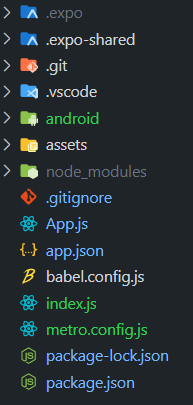
\includegraphics[height=0.5\textwidth]{Theorie/ReactNative/ExpoEject.png}
    \caption{Expo Eject Änderungen}
  \end{center}
\end{figure}

\begin{itemize}
  \item 
\end{itemize}

Um das Projekt für iOS-Geräte zu konfigurieren, führt man folgenden Befehl auf einem MacOS-PC aus:

\begin{lstlisting}
C:\example\expoInitBlank> npx pod-install
\end{lstlisting}

